\documentclass[10pt,UTF8]{ctexart}

\usepackage[margin=0.72in]{geometry}
\usepackage{microtype}
\usepackage{graphicx}
\usepackage{subcaption}
\usepackage{booktabs}
\usepackage{array}
\usepackage{tabularx}
\usepackage[hidelinks]{hyperref}
\usepackage{xcolor}
\usepackage{enumitem}
\usepackage{amsmath}
\usepackage{dblfloatfix}
\usepackage{float}
\usepackage{setspace}

\graphicspath{{../results/arch_compare_20260526/}}

\setlength{\columnsep}{0.22in}
\setlength{\parindent}{0pt}
\setlength{\parskip}{0.45em}
\renewcommand{\arraystretch}{1.12}
\setlist[itemize]{leftmargin=1.2em,itemsep=0.2em,topsep=0.25em}
\makeatletter
\setlength{\@fptop}{0pt}
\setlength{\@fpbot}{0pt plus 1fil}
\setlength{\@fpsep}{8pt}
\makeatother

\definecolor{PaperBlue}{HTML}{203A63}
\definecolor{PaperOrange}{HTML}{F59E0B}
\definecolor{PaperGray}{HTML}{5B6578}
\definecolor{PaperLight}{HTML}{F8FAFC}

\title{\vspace{-1.1em}\bfseries 十种遗忘注意力机制的参考实现 \\ \large (Reference Implementations of 10 Forgetting Attention Mechanisms)}
\author{Vuk Rosic\\\small 独立研究项目 (Independent Research Project)\\\small 代码 (Code): \url{https://github.com/vukrosic/forgetting-attention}}
\date{2026 年 5 月 26 日}

\begin{document}
\maketitle

\begin{abstract}
我们梳理并实现了十种用于因果注意力 (causal attention) 的遗忘与记忆策略 (forgetting and memory policies),
并为每一种提供了易读的 PyTorch 参考实现 (reference implementation),
同时附带可将其扩展到更大模型与更长训练预算的训练与评估基础设施 (training and evaluation infrastructure)。
作为初步验证,我们在三种上下文长度 (context length, 即 2K、4K、8K) 下,
在一个 18M 参数级别 (18M-class) 的 LLM transformer 上,
用单张 RTX 3090 各跑 5 分钟,运行了全部 11 种机制 (稠密注意力 dense 加上 10 种变体)。
在这个小规模、无融合内核 (unfused) 的设置下,
稠密注意力 (dense) 在验证损失 (validation loss) 与吞吐量 (throughput) 上都领先;
在记忆变体中,最简单的几种 —— 块均值压缩 (block-mean compression)、年龄衰减 (age decay)、
分层摘要 (hierarchical summaries)、惊讶度保留 (surprise retention) —— 聚集在第二梯队。
随着上下文长度的增加,遗忘机制 (forgetting mechanism) 的吞吐量相对优势逐渐显现:
在 2K 上下文长度下,稠密的速度大约是最强遗忘机制的两倍,但在 8K 时差距缩小到约 15\%,
这暗示进一步的扩展 (scaling) 可能会让排名反转。
\end{abstract}

\begin{figure}[H]
\centering
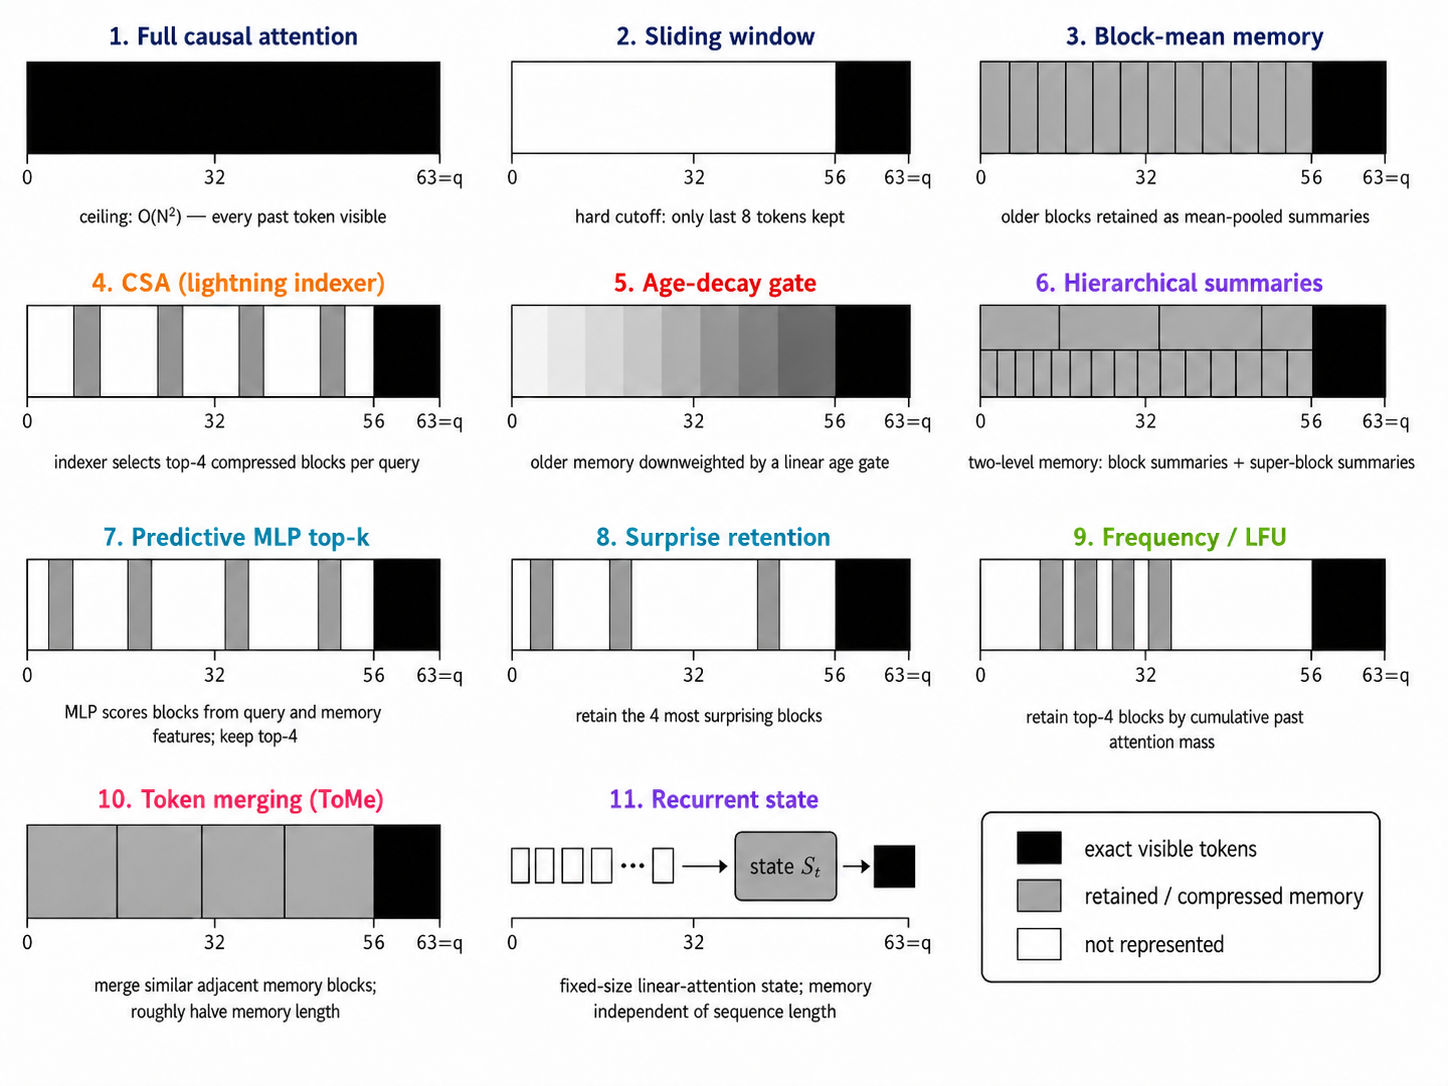
\includegraphics[width=0.82\textwidth]{mechanism_diagrams.png}
\caption{本文涉及的各机制的记忆示意图。黑色区域 (black) 表示查询 (query) 可以完整访问;
灰色区域 (gray) 表示通过记忆或门控 (memory/gating) 保留下来的部分;
白色区域 (white) 表示已经在可见记忆之外的部分。}
\label{fig:diagrams}
\end{figure}

\section{相关工作 (Literature Review)}

长上下文 transformer (long-context transformers) 通常会改变以下四件事中的一件:
哪些 token 可以被注意到、过去的状态如何存储、旧信息如何被检索、
或在注意力运行之前如何降低序列长度 (sequence length)。
诸如 Longformer、BigBird、Reformer、Routing Transformer 等
局部与稀疏注意力方法 (local and sparse attention)
减少了每个查询 (query) 需要比对的键 (key) 的数量~\cite{longformer,bigbird,reformer,routing_transformer}。
而 Transformer-XL、Compressive Transformer 等记忆系统 (memory systems)
则跨段携带状态,或对即将离开窗口的旧状态进行压缩~\cite{transformer_xl,compressive_transformer}。
kNN-LM、Memorizing Transformers 等检索方法 (retrieval methods)
则把部分记忆外置到一个数据存储 (datastore) 中~\cite{knn_lm,memorizing_transformers}。

现代大型模型也很重视记忆压缩 (memory compression)。
DeepSeek-V2 和 DeepSeek-V3 使用多头潜在注意力 (Multi-head Latent Attention, MLA)
来在大规模下降低 KV 缓存 (KV-cache) 成本~\cite{deepseek_v2,deepseek_v3}。
本文的 CSA 基线就是这一家族中的一个小型参考点 (small reference point):
旧上下文仍然作为注意力的材料 (attention material),
但在被注意力读取之前会以更便宜的方式表示。
ToMe 等 token 合并 (token-merging) 工作提出了另一种原语:
通过合并而不是仅靠遮蔽 (masking) 或丢弃 (dropping) 来压缩冗余内容~\cite{tome}。

\section{研究目标 (Goal)}

\begin{itemize}
\item 提供 10 种遗忘注意力策略的参考实现 (reference implementation),
便于内核编写者 (kernel writers) 与后续实验进行扩展。
\item 通过数学、代码与示意图清楚地解释每一种思想。
\item 提供初步分析与实验配置。
\end{itemize}

\section{对比的策略 (Policies Compared)}

每一种策略都是同一 transformer 块 (transformer block) 内
可替换的逐层注意力模块 (per-layer attention module)。
图~\ref{fig:diagrams} 展示了每种机制在最后一个查询位置 (last query position)
上的注意力模式 (attention pattern) 是什么样子的。

\begin{itemize}
\item \textbf{dense} (经典基线 classic baseline) ---
完整的因果 SDPA (full causal SDPA),配合 GQA (grouped-query attention) 与 RoPE。
每个 token 都对所有更早的 token 进行注意,因此代价随上下文长度二次增长 (quadratic)。
\item \textbf{local} --- 窗口大小为 $W=64$ 的滑动窗口 (sliding window),不带记忆。
作为孤立的基线 (isolated baseline) 引入,以便其他所有策略
(它们都包含局部注意力加上额外记忆机制) 可以与纯局部进行对比:
额外的记忆机制是否真的有用,还是局部注意力本身就承担了大部分工作?
\item \textbf{compressed\_memory} --- 块均值压缩 (block-mean compression),所有块都可见,无门控。
远距离的上下文被表示为每个固定大小的键/值块 (key/value block) 的均值,
因此每个查询读取的是过去的简短摘要再加上一个新鲜的局部窗口 (local window)。
\item \textbf{csa} --- 闪电索引器 (lightning indexer) 对压缩块进行打分;
每个查询保留 top $k=4$ 的块 (DeepSeek V4 风格的压缩稀疏注意力 compressed sparse attention)。
一个小的逐查询 MLP (per-query MLP) 给块摘要 (block summaries) 打分,
只有得分最高的块会贡献到输出,其余的会被遮蔽掉。
\item \textbf{age\_forgetting} --- 在压缩块上施加线性年龄衰减门 (linear age-decay gate):
门 $=1-r\cdot \text{age}$。较旧的摘要权重会平滑地衰减直至消失,
给出一种软性的最近性偏好 (soft recency prior),
而不需要选定一个硬性的窗口截断 (hard window cutoff)。
\item \textbf{hierarchical} --- 两层 (two-level):块与块的超级块 (super-blocks-of-blocks),
每一层都被 $1/(\text{level}+1)$ 门控。
模型可以同时读取精细的局部摘要 (fine local summaries) 与
更粗粒度的远距离摘要 (coarser distant summaries),信息越远每个 token 的代价越低。
\item \textbf{predictive} --- 一个小型 MLP 根据 $(Q, K_b, \text{age})$ 给每个块打分;
保留 top-$k$。与上面那些固定打分规则 (fixed scoring rules) 不同,
这个路由器 (router) 端到端地学习每个查询需要哪些块。
\item \textbf{surprise\_retention} (新增) ---
每个块的、与查询无关 (query-independent) 的打分
$s_b = \|V_b - f(K_b)\|^2$,其中 $f$ 是一个学习到的预测器 (learned predictor);
保留 top-$k$ 最让人意外 (most-surprising) 的块。
那些值能轻易从自身键预测出的块被当作冗余 (redundant) 丢弃,
只有信息量大的块 (information-rich blocks) 才能保留下来。
\item \textbf{frequency\_lfu} (新增) ---
打分是过去每个块上注意力质量 (attention mass) 的因果累积和 (causal cumulative sum):
模型实际用过的块会被保留下来。
保留是一个自组织 (self-organizing) 的过程 ---
训练期间的使用情况决定了哪些会留在记忆里。
\item \textbf{token\_merge} (新增) ---
在记忆上进行二部图内容相似度合并 (bipartite content-similarity merge):
每隔一个块就与其邻居配对,合并相似度 top-$r$ 的对,
使记忆长度减半。这一思想改编自视觉领域的 ToMe:
通过合并相似内容来压缩冗余,而不是丢弃或遮蔽。
\item \textbf{recurrent\_state} (新增) ---
线性注意力 (linear attention),使用正特征映射 (positive feature map) $\phi$
和因果累积状态 (causal cumulative state)
$S_t = \sum_{s\leq t} \phi(K_s)\otimes V_s$。
每层的记忆是 $O(d_k^2)$,与 $T$ 无关。
过去的 token 永远不会被重新读取,它们完全活在一个固定大小的累加器 (fixed-size accumulator) 里,
由模型每一步往前滚动 (roll forward)。
\end{itemize}

\section{正确性测试套件 (Correctness Suite)}

每一种机制在进入扫描 (sweep) 之前都要通过五项 CUDA 测试:
形状/数据类型 (shape/dtype)、因果性 (causality,
即对未来位置的扰动不应改变更早位置的输出)、
遮蔽正确性 (mask correctness)、梯度流 (gradient flow)、
以及峰值显存 (peak memory) 的记录。
当前状态:在一张 RTX 3090 上 55/55 全部通过。
运行方式:\verb|python -m tests.test_forgetting_mechanisms|。

\section{实验配置 (Setup)}

\begin{table}[H]
\centering
\small
\caption{扩展扫描 (scaling sweep) 的共享实验配置。}
\label{tab:setup}
\begin{tabular}{@{}ll@{}}
\toprule
项目 (Item) & 取值 (Value) \\
\midrule
配置预设 (Config preset) & \texttt{CSAMinimumPaperConfig} \\
参数量 (Parameters) & 18.35M--18.77M \\
隐藏维度 (Hidden size) & 256 \\
层数 / 头数 (Layers / heads) & 8 / 8 \\
KV 头数 (KV heads, GQA) & 4 \\
上下文长度扫描 (Context length sweep) & \{2048, 4096, 8192\} \\
批大小 (Batch size, 已调) & 4 / 2 / 1 (每步 token 数保持不变) \\
优化器 (Optimizer) & Muon (矩阵) + AdamW (其他) \\
数据集 (Dataset) & \texttt{processed\_data/speedrun\_40M} \\
硬件 (Hardware) & 1$\times$NVIDIA RTX 3090, 24GB \\
单次预算 (Budget per run) & 300 秒有效训练时间 (active training seconds) \\
评估频率 (Eval cadence) & 每 200 步 \\
随机种子 (Seeds) & 1 (本次运行) \\
\bottomrule
\end{tabular}
\end{table}

\textbf{公平性规则 (Fairness rule)}。各行之间只有逐层注意力模块发生变化;
模型、数据、优化器、随机种子、硬件都完全一致。
批大小随上下文长度调整,以保持每步 token 数恒定为 8192,
每次运行被限制在 300 秒有效训练时间内。

\textbf{指标 (Metrics)}。每次运行都会写入 \texttt{metrics.json},
包含最终验证损失 (final validation loss)、已见 token 数 (tokens seen)、
吞吐量 tok/s、有效时间 (active time) 与挂钟时间 (wall time)、
峰值已分配 / 已预留显存 (peak allocated/reserved VRAM),
以及按评估点记录的相对 token 与秒数的损失历史。

\section{结果 (Results)}

在我们的设置下 (一张 RTX 3090,18M 参数级 transformer,300 秒预算,
单种子,无融合的 PyTorch),33 次运行的扫描在不同上下文长度下给出了一致的模式。
稠密注意力 (dense) 在验证损失与吞吐量上都领先。
局部注意力 (local) 是最强的廉价基线。
压缩记忆 (compressed-memory) 家族紧跟在 local 后面;
CSA 与循环状态 (recurrent state) 在如此短的预算下排得更靠后。
在遗忘规则中,最简单的几个表现最好:
2K 与 4K 时是年龄衰减 (age decay) 与不加门控的压缩记忆 (ungated compressed memory),
8K 时是惊讶度保留 (surprise retention)。
学习型预测路由器 (learned predictive router) 与 token 合并 (token-merge) 变体
在这里相对较弱 —— 这是一个信号:
在无融合内核、短预算的设置下,额外的选择机制 (selection machinery)
可能反而输给更简单的记忆规则。

\begin{table}[H]
\centering
\scriptsize
\caption{完成的 33 次运行扫描。每一行是在同一张 RTX 3090 上跑的一次 300 秒运行。
最终损失并不是唯一公平的视角,因为更快的机制在时间上限内能处理更多的 token。}
\label{tab:results}
\resizebox{\textwidth}{!}{\begin{tabular}{@{}llrrrrr@{}}
\toprule
Context & Mechanism & Val loss & Tokens (M) & Tok/s & Time (s) & VRAM GiB \\
\midrule
2048 & \texttt{age\_forgetting} & 4.7595 & 13.9 & 45.7k & 305 & 9.91 \\
2048 & \texttt{compressed\_memory} & 4.7677 & 14.0 & 45.8k & 305 & 9.90 \\
2048 & \texttt{csa} & 5.2627 & 17.7 & 58.3k & 303 & 7.66 \\
2048 & \texttt{dense} & 4.3386 & 37.7 & 124.1k & 304 & 6.94 \\
2048 & \texttt{frequency\_lfu} & 4.7890 & 13.1 & 42.7k & 306 & 9.91 \\
2048 & \texttt{hierarchical} & 4.7589 & 13.9 & 45.4k & 305 & 11.38 \\
2048 & \texttt{local} & 4.5106 & 27.9 & 91.6k & 304 & 7.00 \\
2048 & \texttt{predictive} & 4.8816 & 10.9 & 35.4k & 307 & 12.15 \\
2048 & \texttt{recurrent\_state} & 5.5019 & 18.0 & 59.1k & 305 & 7.00 \\
2048 & \texttt{surprise\_retention} & 4.7906 & 13.4 & 43.7k & 306 & 9.91 \\
2048 & \texttt{token\_merge} & 4.7969 & 12.9 & 42.3k & 306 & 9.89 \\
4096 & \texttt{age\_forgetting} & 4.8268 & 13.1 & 43.1k & 304 & 5.76 \\
4096 & \texttt{compressed\_memory} & 4.8275 & 13.1 & 43.2k & 303 & 5.76 \\
4096 & \texttt{csa} & 5.5567 & 10.3 & 34.1k & 302 & 3.88 \\
4096 & \texttt{dense} & 4.5522 & 26.9 & 89.4k & 301 & 3.51 \\
4096 & \texttt{frequency\_lfu} & 4.8611 & 12.3 & 40.4k & 303 & 5.76 \\
4096 & \texttt{hierarchical} & 4.8367 & 13.1 & 43.2k & 303 & 5.74 \\
4096 & \texttt{local} & 4.6212 & 24.5 & 81.4k & 301 & 3.57 \\
4096 & \texttt{predictive} & 4.9611 & 10.1 & 33.3k & 304 & 6.13 \\
4096 & \texttt{recurrent\_state} & 5.6000 & 15.4 & 50.9k & 303 & 3.54 \\
4096 & \texttt{surprise\_retention} & 4.8577 & 12.7 & 41.9k & 303 & 5.76 \\
4096 & \texttt{token\_merge} & 4.9331 & 10.4 & 34.3k & 303 & 5.75 \\
8192 & \texttt{age\_forgetting} & 5.0689 & 9.8 & 32.5k & 302 & 2.93 \\
8192 & \texttt{compressed\_memory} & 5.0733 & 9.7 & 32.3k & 302 & 2.93 \\
8192 & \texttt{csa} & 5.8409 & 5.0 & 16.7k & 302 & 2.00 \\
8192 & \texttt{dense} & 4.9768 & 13.9 & 46.2k & 301 & 1.80 \\
8192 & \texttt{frequency\_lfu} & 5.1016 & 9.2 & 30.4k & 302 & 2.93 \\
8192 & \texttt{hierarchical} & 5.1066 & 9.0 & 29.9k & 302 & 2.92 \\
8192 & \texttt{local} & 4.9923 & 12.7 & 42.3k & 301 & 1.86 \\
8192 & \texttt{predictive} & 5.1282 & 7.8 & 25.8k & 302 & 3.51 \\
8192 & \texttt{recurrent\_state} & 5.7510 & 11.9 & 39.6k & 302 & 1.82 \\
8192 & \texttt{surprise\_retention} & 5.0660 & 9.2 & 30.6k & 302 & 2.93 \\
8192 & \texttt{token\_merge} & 5.1591 & 7.5 & 24.9k & 302 & 2.92 \\
\bottomrule
\end{tabular}
}
\end{table}

\begin{figure}[H]
\centering
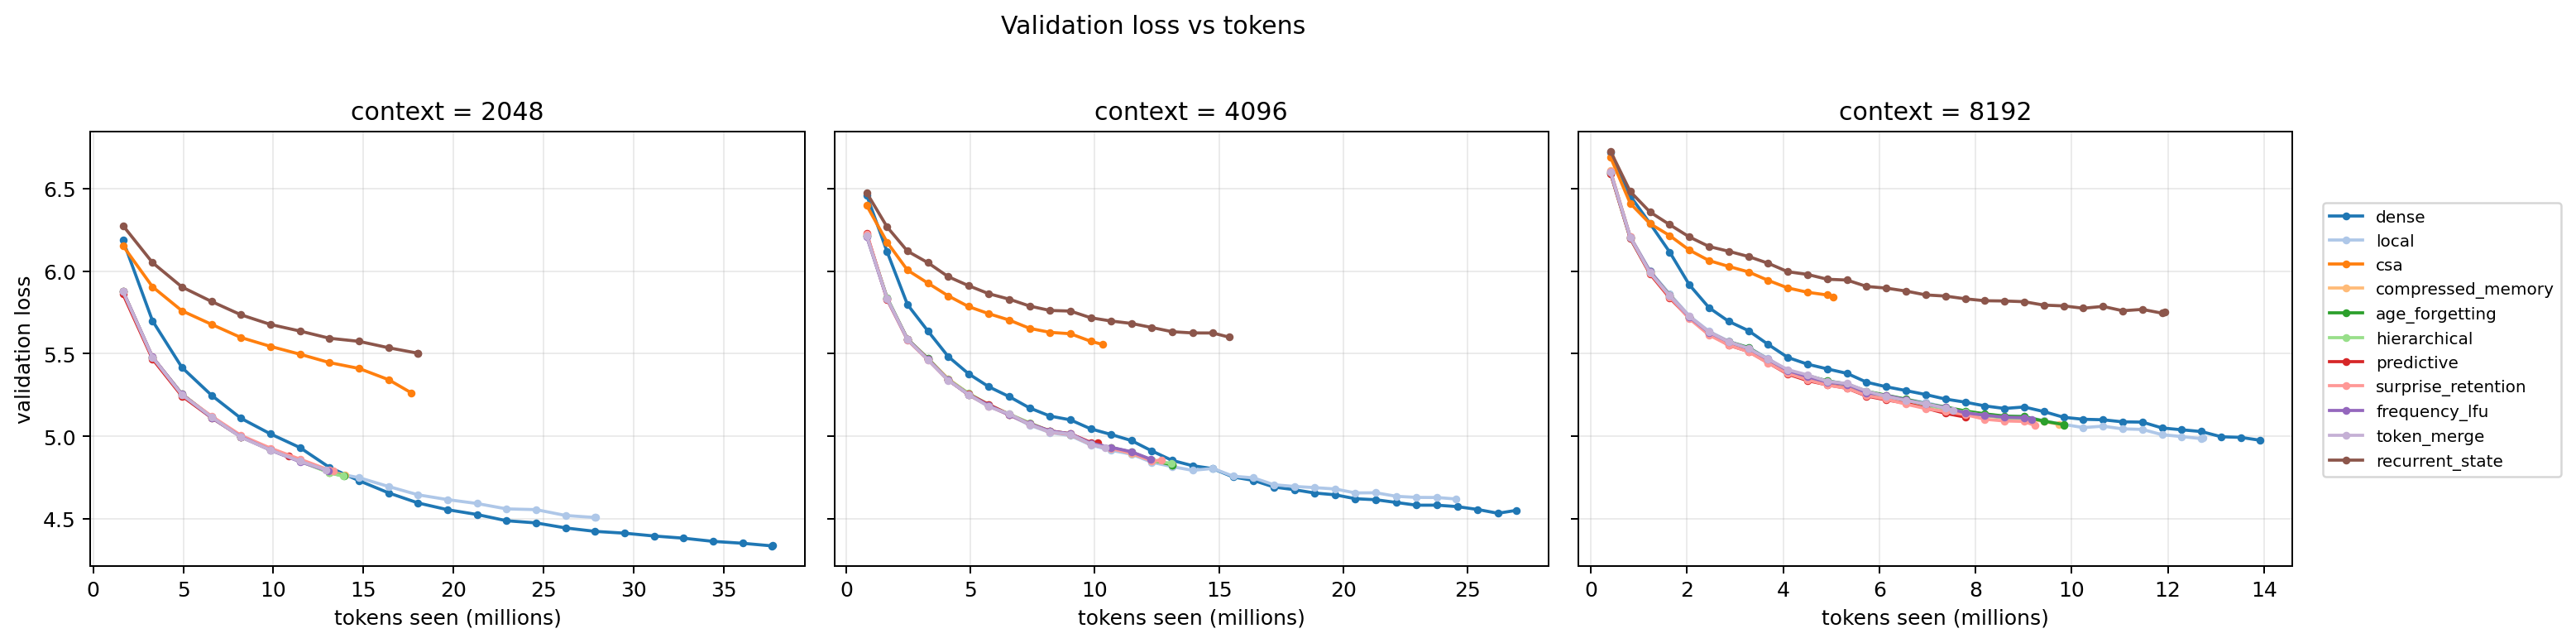
\includegraphics[width=\textwidth]{../results/forgetting_scaling_latest/loss_vs_tokens.png}
\caption{验证损失 (validation loss) 相对于已见 token 数 (tokens seen)。
由于扫描有时间上限 (time-capped),这条曲线是最公平的视角。}
\label{fig:val-loss}
\end{figure}

\begin{figure}[H]
\centering
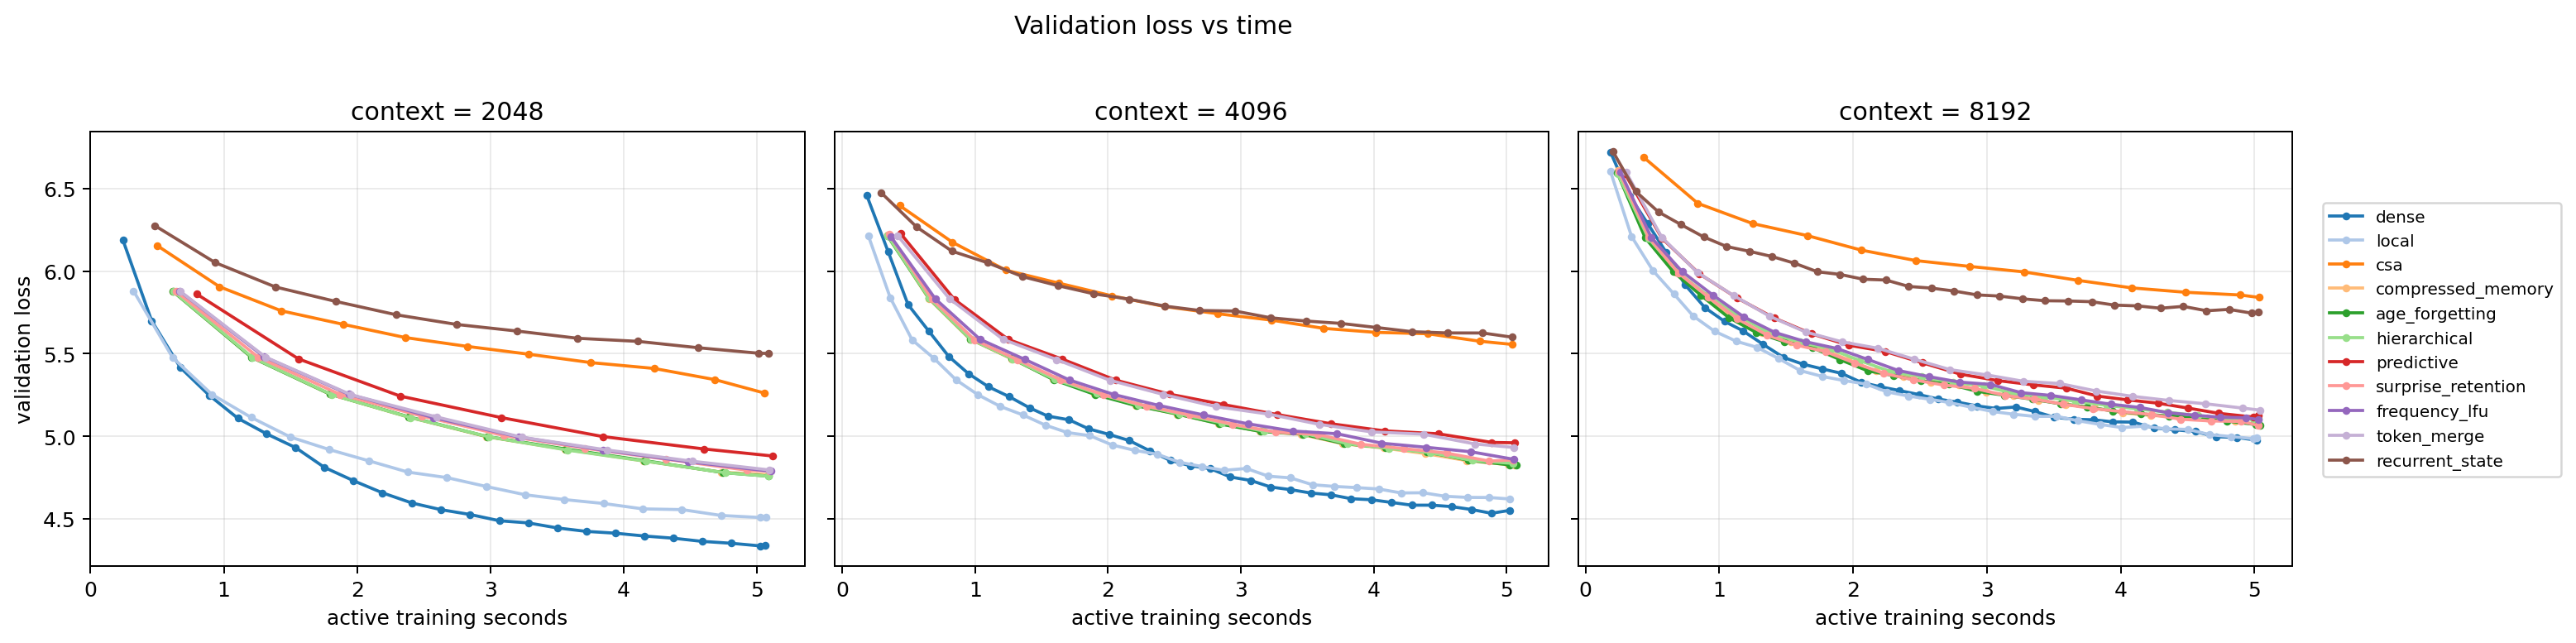
\includegraphics[width=\textwidth]{../results/forgetting_scaling_latest/loss_vs_time.png}
\caption{验证损失相对于有效训练秒数 (active training seconds)。}
\label{fig:loss-time}
\end{figure}

\begin{figure}[H]
\centering
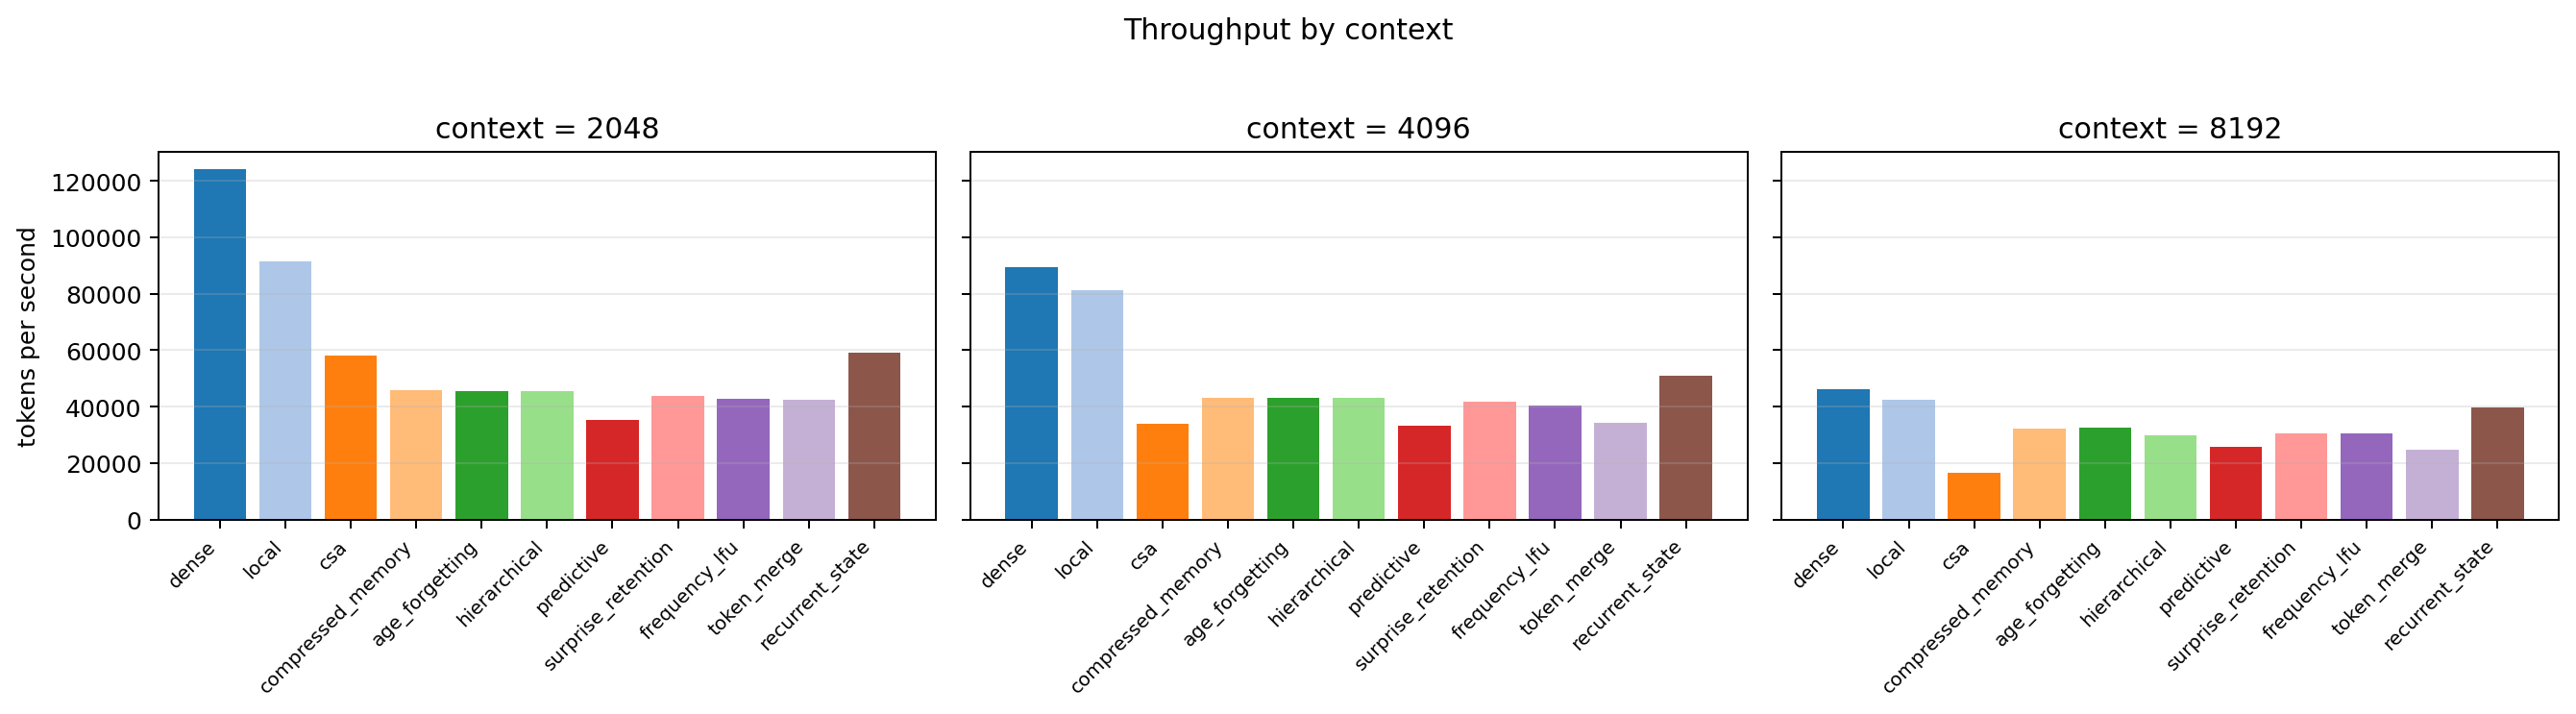
\includegraphics[width=\textwidth]{../results/forgetting_scaling_latest/throughput_by_context.png}
\caption{按上下文长度划分的吞吐量 (throughput, tokens/second)。}
\label{fig:throughput-context}
\end{figure}

\begin{figure}[H]
\centering
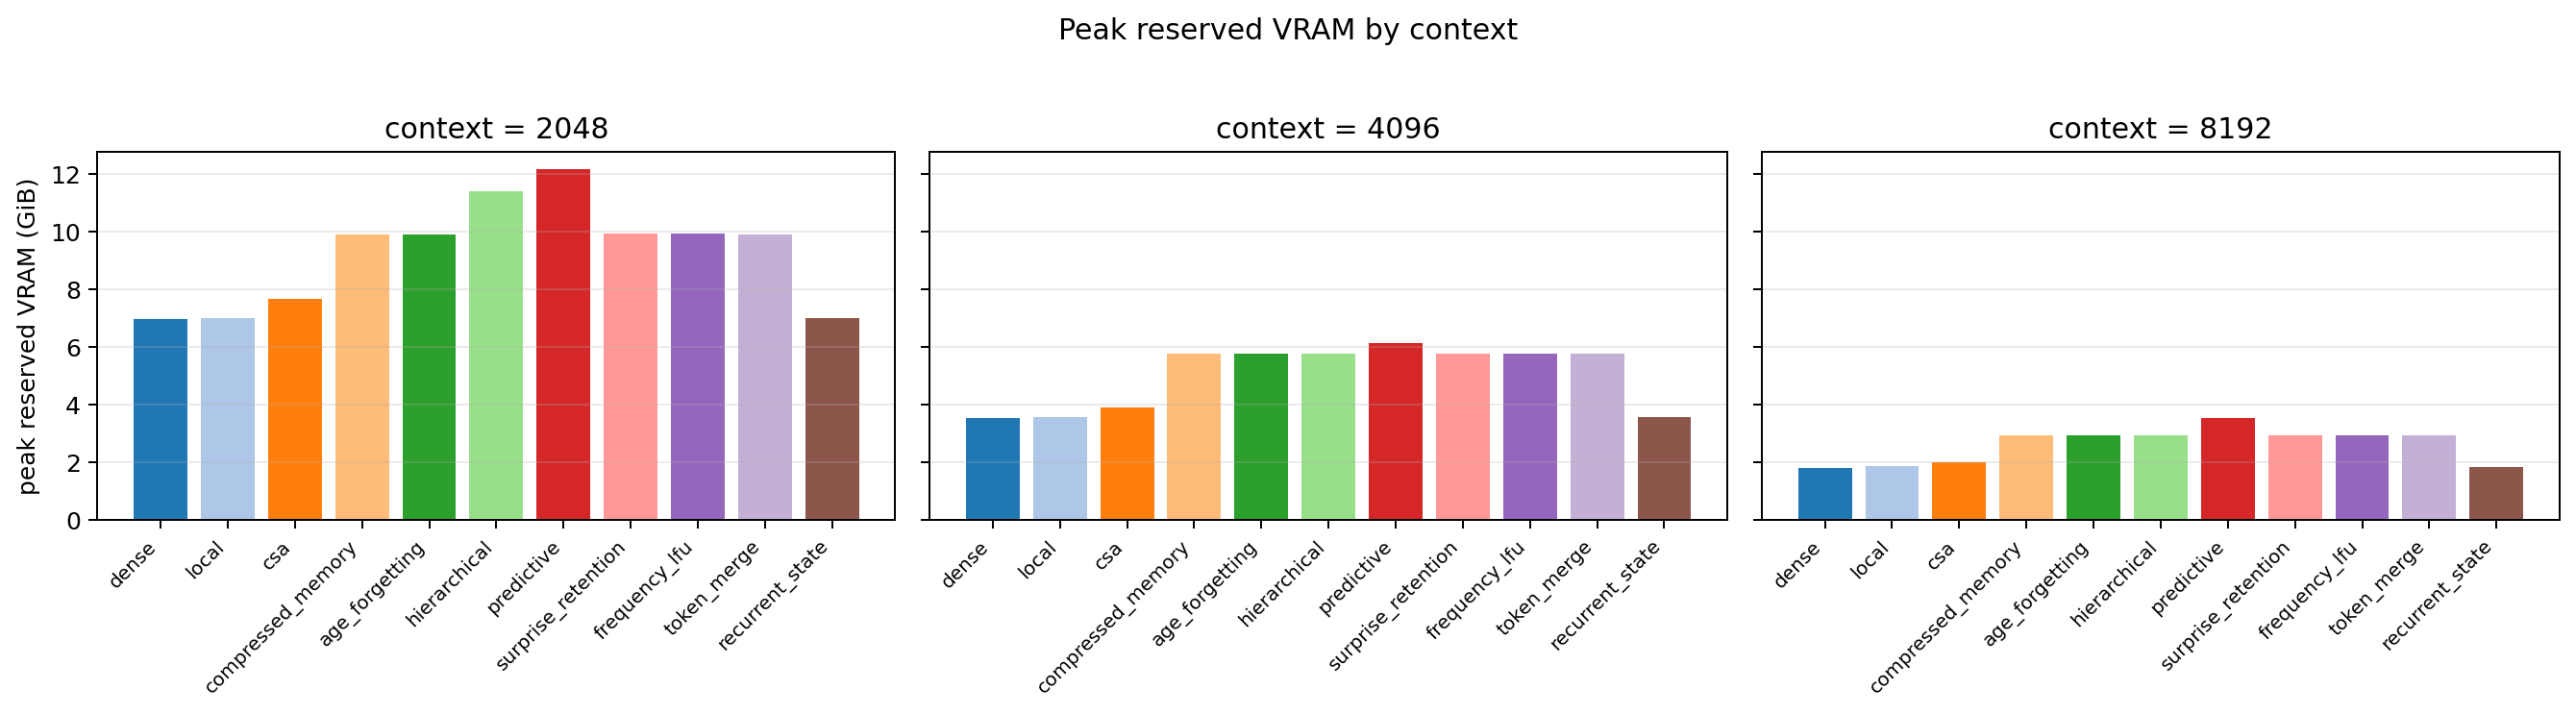
\includegraphics[width=0.85\textwidth]{../results/forgetting_scaling_latest/vram_by_context.png}
\caption{按上下文长度划分的峰值已预留显存 (peak reserved VRAM)。}
\label{fig:vram-context}
\end{figure}

\textbf{对我们这套设置的结论 (Takeaway for our setup)}。
在这次参考运行中,遗忘策略 (forgetting policies) 在两个指标上都没有击败 dense 或 local。
但图~\ref{fig:throughput-context} 表明吞吐量差距 (throughput gap) 随上下文长度迅速缩小:
在 2K 时,dense (124K tok/s) 大约是最强遗忘机制的两倍快;
在 4K 时差距缩小到约 1.7$\times$;
在 8K 时,dense (46K tok/s) 仅比 recurrent state (40K tok/s) 快约 15\%,
压缩记忆变体也类似地逼近 dense。
dense 随序列长度二次增长 (quadratically),而遗忘机制更接近线性增长 (linear),
因此自然的下一步 —— 更长的上下文或更大的模型 ——
正是这些策略本来就被设计去取胜 (win on throughput) 的吞吐量区域;
一旦如此,按时间的损失视角 (loss-per-second, 图~\ref{fig:loss-time})
也会随之反转到它们一边。

\section{扩展路径 (Scaling Path)}

每一种策略都是带有数学注释的纯 PyTorch 模块 (plain-PyTorch module),
并配有通过的因果性测试 (causal correctness test),
因此一个内核编写者 (kernel writer) 可以把它移植到 Triton 或 CUDA,
与参考实现进行 A/B 对比以验证精确性 (A/B for exactness),
并在更大规模上重新跑这套扫描。
训练脚本是以单 GPU 优先 (single-GPU first) 写的,
但配置 (config)、检查点 (checkpoints) 和 \texttt{metrics.json} 的格式
无需改代码就能适配 \texttt{torchrun}、DDP 或公司内部的训练框架 (internal harness)。

\section{局限 (Limitations)}

单一随机种子、单一 3090、单一数据集、单一参数规模、未融合的内核。
这些数字描述的是每种机制在这一具体设置下达到平台期 (plateau) 的样子。
任务是普通的下一 token 预测 (next-token prediction),
可能对记忆系统的压力不够,无法暴露出旧信息何时是有用的。
一次融合内核 (fused-kernel) 的重新运行,
或一个长记忆检索任务 (long-memory retrieval task) 都可能改变排名。

\section{产出 (Output Artifacts)}

代码 (Code): \url{https://github.com/vukrosic/forgetting-attention}。
四种新机制位于 \path{models/new_forgetting.py},
正确性测试套件位于 \path{tests/test_forgetting_mechanisms.py},
扩展扫描位于 \path{experiments/forgetting_scaling_sweep.py}。

\section{结论 (Conclusion)}

这次扫描把十种记忆思想转化成了可运行的、保持因果性的 PyTorch 模块,
配有通过的正确性测试和一份完整的等时间扩展表 (equal-time scaling table)。
在这次 18M 参考运行中,dense 与 local 领先;
在记忆家族中,age decay、不加门控的 compressed memory 和 surprise retention
是最值得融合 (fuse) 并重新跑的候选。

\section{下一步 (Next Steps)}

\begin{itemize}
\item 扩展算力 (scale compute,包括更大的模型、更长的训练预算、更多的随机种子),
看哪些策略仍然有前景。
\item 如果在扩展之后还有策略能撑住,就为这些路径写融合内核 (fused kernels)。
\end{itemize}

\begingroup
\small
\setstretch{0.92}
\setlength{\itemsep}{0pt}
\begin{thebibliography}{13}
\bibitem{deepseek_v2}
DeepSeek-AI.
\newblock {\em DeepSeek-V2: A Strong, Economical, and Efficient Mixture-of-Experts Language Model}.
\newblock 2024.

\bibitem{deepseek_v3}
DeepSeek-AI.
\newblock {\em DeepSeek-V3 Technical Report}.
\newblock 2024.

\bibitem{csaminipaper}
V.~Rosic.
\newblock {\em Can Compressed Sparse Attention Help Under Equal GPU Time?}
\newblock Internal research report, May 24, 2026.

\bibitem{transformer_xl}
Z.~Dai, Z.~Yang, Y.~Yang, J.~Carbonell, Q.~Le, and R.~Salakhutdinov.
\newblock {\em Transformer-XL: Attentive Language Models Beyond a Fixed-Length Context}.
\newblock ACL 2019.

\bibitem{compressive_transformer}
J.~W. Rae, A.~Potapenko, S.~J. Kayumov, and T.~P. Lillicrap.
\newblock {\em Compressive Transformers for Long-Range Sequence Modelling}.
\newblock ICLR 2020.

\bibitem{longformer}
I.~Beltagy, M.~E. Peters, and A.~Cohan.
\newblock {\em Longformer: The Long-Document Transformer}.
\newblock arXiv:2004.05150, 2020.

\bibitem{bigbird}
M.~Zaheer et al.
\newblock {\em Big Bird: Transformers for Longer Sequences}.
\newblock NeurIPS 2020.

\bibitem{reformer}
N.~Kitaev, L.~Kaiser, and A.~Levskaya.
\newblock {\em Reformer: The Efficient Transformer}.
\newblock ICLR 2020.

\bibitem{routing_transformer}
A.~Roy, M.~Saffar, A.~Vaswani, and D.~Grangier.
\newblock {\em Efficient Content-Based Sparse Attention with Routing Transformers}.
\newblock TACL 2021.

\bibitem{memorizing_transformers}
Y.~Wu, M.~N. Rabe, D.~Hutchins, and C.~Szegedy.
\newblock {\em Memorizing Transformers}.
\newblock ICLR 2022.

\bibitem{knn_lm}
U.~Khandelwal, O.~Levy, D.~Jurafsky, L.~Zettlemoyer, and M.~Lewis.
\newblock {\em Generalization through Memorization: Nearest Neighbor Language Models}.
\newblock ICLR 2020.

\bibitem{tome}
D.~Bolya, C.-Y.~Fu, X.~Dai, P.~Zhang, C.~Feichtenhofer, J.~Hoffman.
\newblock {\em Token Merging: Your ViT But Faster}.
\newblock ICLR 2023.

\bibitem{linear_attn}
A.~Katharopoulos, A.~Vyas, N.~Pappas, F.~Fleuret.
\newblock {\em Transformers are RNNs: Fast Autoregressive Transformers with Linear Attention}.
\newblock ICML 2020.
\end{thebibliography}
\endgroup

\end{document}
